\documentclass[12pt,a4paper]{article}

% 1. ENCODING & LANGUAGE
\usepackage[utf8]{inputenc}
\usepackage[T1]{fontenc}
\usepackage[romanian]{babel}
\usepackage{float}
\usepackage{listings}
\usepackage{xcolor}
\usepackage{forest}
\usepackage{tikz}
\usetikzlibrary{shapes.geometric, arrows.meta, positioning,calc}

\lstset{
    inputencoding=utf8,
    extendedchars=true,
    literate={├}{|}1 {─}{--}1 {└}{+}1
}

% Definire limbaj JavaScript/TypeScript
\lstdefinelanguage{TypeScript}{
  keywords={typeof, new, true, false, catch, function, return, null, catch, switch, var, if, in, while, do, else, case, break, interface, type, export, default, const, let, import, from},
  keywordstyle=\color{blue}\bfseries,
  ndkeywords={class, boolean, throw, implements, this, string, number, any, useState, useEffect, useRef},
  ndkeywordstyle=\color{teal}\bfseries,
  identifierstyle=\color{black},
  sensitive=false,
  comment=[l]{//},
  morecomment=[s]{/*}{*/},
  commentstyle=\color{purple}\ttfamily,
  stringstyle=\color{red}\ttfamily,
  morestring=[b]',
  morestring=[b]"
}

% Definire limbaj Python
\lstdefinelanguage{Python}{
  keywords={def, class, return, if, elif, else, while, for, in, try, except, import, from, as, True, False, None, and, or, not, is},
  keywordstyle=\color{blue}\bfseries,
  ndkeywords={self, models, CharField, ForeignKey, IntegerField, TextField, JSONField, DateTimeField},
  ndkeywordstyle=\color{teal}\bfseries,
  identifierstyle=\color{black},
  sensitive=true,
  comment=[l]{\#},
  commentstyle=\color{gray}\ttfamily,
  stringstyle=\color{red}\ttfamily,
  morestring=[b]',
  morestring=[b]"
}

% 2. PAGE LAYOUT & GEOMETRY
\usepackage[a4paper,
    top=2.5cm,
    bottom=2.5cm,
    left=3cm,
    right=2.5cm,
    headheight=15pt,
    footskip=1cm]{geometry}

% 3. PROFESSIONAL TYPOGRAPHY
\usepackage{newtxtext, newtxmath} % Times New Roman alternative with better math
\usepackage{microtype} % Micro-typographic improvements
\usepackage{setspace}
\onehalfspacing

% 4. MATHEMATICS & SCIENCE
\usepackage{amsmath, amssymb, amsthm}
\usepackage{bm} % Bold math symbols

% 5. GRAPHICS & TABLES
\usepackage{graphicx}
\usepackage{booktabs} % Professional tables
\usepackage{array} % Extended array functionality
\usepackage{caption} % Better captions
\captionsetup{font=small, labelfont=bf}

% 6. REFERENCES & HYPERLINKS
\usepackage{hyperref}
\hypersetup{
    colorlinks=true,
    linkcolor=blue,
    citecolor=blue,
    urlcolor=blue,
    pdfauthor={Alexandru PONTOȘ},
    pdftitle={Sistem de inventariere și monitorizare a echipamentelor dintr-un datacenter},
    pdfsubject={Cercetare științifică}
}

% 7. HEADERS & FOOTERS
\usepackage{fancyhdr}
\pagestyle{fancy}
\fancyhf{}
\fancyhead[L]{\small\textsc{Inventariere și Monitorizare Datacenter}}
\fancyhead[R]{\small\textsc{\nouppercase{\leftmark}}}
\fancyfoot[C]{\thepage}
\renewcommand{\headrulewidth}{0.4pt}
\renewcommand{\footrulewidth}{0pt}

% 8. SECTION FORMATTING
\usepackage{titlesec}
\titleformat{\section}
    {\normalfont\Large\bfseries}
    {\thesection}{1em}{}
\titleformat{\subsection}
    {\normalfont\large\bfseries}
    {\thesubsection}{1em}{}
\titleformat{\subsubsection}
    {\normalfont\normalsize\bfseries}
    {\thesubsubsection}{1em}{}

% 9. ABSTRACT ENVIRONMENT
\usepackage{abstract}
\renewcommand{\abstractname}{\vspace{-\baselineskip}}
\setlength{\absleftindent}{0pt}
\setlength{\absrightindent}{0pt}

% 10. CUSTOM COMMANDS
\newcommand{\keyword}[1]{\textbf{#1}}
\newcommand{\todo}[1]{\textcolor{red}{[TODO: #1]}}

% ============================================================================
% DOCUMENT START
% ============================================================================

\begin{document}

% TITLE PAGE
\begin{titlepage}
    \centering
    
    % Logo (uncomment and add your logo)
    % \vspace*{0.5cm}
    % \includegraphics[width=0.3\textwidth]{logo.png}
    
    \vspace*{2cm}
    
    {\LARGE\bfseries Sistem de inventariere și monitorizare\\a echipamentelor dintr-un datacenter}
    
    \vspace{1.5cm}
    
    {\large Documentație tehnică}
    
    \vspace{2cm}
    
    {\large\bfseries Student Sergent Major\\Alexandru PONTOȘ}
    
    \vspace{1.5cm}
    
    \begin{flushleft}
        \textbf{Coordonator științific:}\\
        Lt. Col. dr. ing. Constantin GRUMĂZESCU\\[0.5cm]
    \end{flushleft}
    
    \vfill
    
    {\large 2026}
    
    \vspace{1cm}
\end{titlepage}

% ABSTRACT
\newpage
\phantomsection
\addcontentsline{toc}{section}{Abstract}
\begin{abstract}
    \noindent
    
    Această lucrare prezintă o abordare eficientă pentru digitalizarea și optimizarea proceselor de gestiune a infrastructurii IT dintr-un centru de date. Cercetarea propune un sistem integrat care utilizează tehnologii web moderne și o interfață vizuală intuitivă pentru inventarierea precisă și monitorizarea stării echipamentelor (rack-uri, servere, dispozitive de rețea). Sistemul implementează mecanisme de actualizare în timp real și validare a datelor, având ca obiectiv final eficientizarea operațională și reducerea erorilor umane asociate administrării manuale. Rezultatele preliminare indică o îmbunătățire semnificativă în organizarea resurselor și o reducere substanțială a timpului necesar pentru auditarea și localizarea echipamentelor comparativ cu metodele tradiționale.
    
    Sistemul menționat rulează ca o aplicație modulară într-o arhitectură containerizată bazată pe Docker, utilizând un backend robust dezvoltat în Python (Django) și o interfață reactivă construită cu React, asigurând portabilitate și ușurință în desfășurare.
    
    \vspace{0.5cm}
    \noindent\textbf{Cuvinte-cheie:} datacenter, DCIM, rack, inventariere, Django, React, monitorizare.
\end{abstract}

% TABLE OF CONTENTS
\newpage
\tableofcontents

% LISTS OF FIGURES AND TABLES (optional)
% \listoffigures
% \listoftables

% ============================================================================
% MAIN CONTENT
% ============================================================================

\newpage
\section{Introducere}
\label{sec:introducere}

\hspace{1em} Centrele de date (Datacenters) reprezintă coloana vertebrală a economiei digitale moderne, găzduind infrastructura critică necesară pentru stocarea, procesarea și distribuția volumelor masive de date. Odată cu creșterea exponențială a serviciilor cloud și a cererii de putere de calcul, complexitatea gestionării fizice și logice a acestor centre a crescut dramatic. Gestionarea eficientă a spațiului în rack-uri, a consumului de energie și a localizării precise a echipamentelor a devenit o provocare majoră pentru administratorii de sistem.

Metodele tradiționale de inventariere, bazate adesea pe fișiere Excel sau diagrame statice, s-au dovedit a fi ineficiente și predispuse la erori umane. Lipsa unei vizibilități în timp real asupra capacității disponibile și a configurării fizice poate duce la alocarea ineficientă a resurselor și la timpi crescuți de intervenție în cazul incidentelor. În acest context, lucrarea de față propune dezvoltarea unui sistem software dedicat tip DCIM (Data Center Infrastructure Management) simplificat, care să ofere o vizualizare grafică interactivă și o gestiune centralizată a activelor IT.

\subsection{Obiectivele Lucrării}
\label{subsec:obiective}

\hspace{1em}Scopul principal al proiectului este realizarea unei platforme web care să permită administratorilor modelarea digitală a infrastructurii fizice a unui datacenter. Obiectivele specifice includ: \textbf{digitalizarea inventarului} pentru a centraliza datele și a evita inconsistențele, o \textbf{vizualizare grafică și intuitivă} a rack-urilor (cabinelor metalice), a echipamentelor și a conexiunilor dintre ele și \textbf{portabilitate} astfel încât sistemul să poată fi rulat pe orice platformă capabilă să ruleze serviciul Docker.

\section{Fundamentare Teoretică}
\label{sec:fundamentare}

\subsection{Arhitectura unui Datacenter}
\label{subsec:arhitectura_dc}

Unitatea fundamentală de organizare într-un datacenter este \textbf{Rack-ul} (dulapul de echipamente). Acesta este standardizat conform normelor EIA-310, având o lățime de 19 inch și o înălțime măsurată în unități standard numite \textbf{Rack Units (U)}. Un unit (1U) are înălțimea de 1.75 inch (44.45 mm). Majoritatea echipamentelor IT (servere, unități de stocare, echipamente de rețea) sunt proiectate pentru a ocupa un număr întreg de unități (1U, 2U, 4U etc.).

Gestionarea eficientă a unui datacenter implică nu doar cunoașterea echipamentelor existente, ci și a poziției lor exacte în rack (ex: Rack 3, U15-U16), a spațiului liber rămas și a caracteristicilor de montare (față/spate/mijloc) și conectivitate (portul/porturi ocupate, conexiunile dintre dispozitive).

\subsection{Soluții DCIM}
\label{subsec:dcim}

Software-ul de tip DCIM (Data Center Infrastructure Management) reprezintă convergența dintre managementul IT și cel al facilităților (clădirii). Deși există soluții comerciale complexe, acestea sunt adesea costisitoare și dificile de implementat pentru centre de date mici sau medii. Proiectul de față propune o soluție care pune accent pe ușurința în utilizare.

\section{Arhitectura Sistemului}
\label{sec:arhitectura}

\hspace{1em}Arhitectura sistemului este structurată în două componente fundamentale: (1) platforma de servicii modulare, care oferă infrastructura necesară pentru interacțiunea cu utilizatorul și logica de business, și (2) baza de date relațională, care asigură persistența structurată a informațiilor critice. Această arhitectură decuplată (Frontend vs Backend) permite dezvoltarea și scalarea independentă.

Figura de mai jos prezintă o privire de ansamblu asupra interacțiunii dintre componentele principale.

\begin{figure}[H]
    \centering
    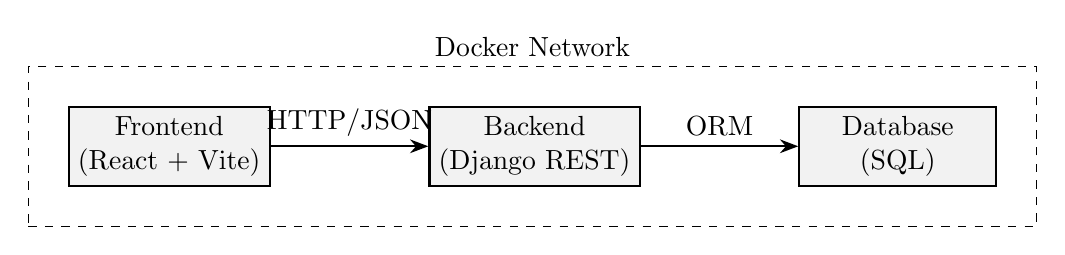
\begin{tikzpicture}[
        node distance=1.5cm,
        component/.style={rectangle, draw=black, thick, minimum width=2.5cm, minimum height=1cm, align=center, fill=gray!10},
        arrow/.style={->, thick, >=Stealth}
    ]
        \node[component] (frontend) {Frontend\\(React + Vite)};
        \node[component, right=2cm of frontend] (backend) {Backend\\(Django REST)};
        \node[component, right=2cm of backend] (db) {Database\\(SQL)};

        \draw[arrow] (frontend) -- node[above] {HTTP/JSON} (backend);
        \draw[arrow] (backend) -- node[above] {ORM} (db);
        
        \node[draw, dashed, inner sep=0.5cm, fit=(frontend) (backend) (db), label=above:Docker Network] (container) {};
    \end{tikzpicture}
    \caption{Diagrama arhitecturală a sistemului propus}
    \label{fig:arhitectura}
\end{figure}

\subsection{Platforma Modulară}
\label{subsec:platforma}

\hspace{1em}Platforma constituie nucleul aplicației și este proiectată pentru a asigura modularitate, scalabilitate și izolare între componente prin utilizarea Docker. Fiecare serviciu (Frontend, Backend, Baza de Date) rulează într-un container propriu, facilitând gestionarea resurselor și portabilitatea.

Arhitectura platformei încorporează următoarele subsisteme:
\begin{enumerate}
    \item \textbf{Frontend (Interfața Client):} Responsabil pentru randarea vizuală a echipamentelor și comunicarea cu utilizatorul.
    \item \textbf{Backend (Serverul API):} Gestionează logica de business și securitatea accesului la date.
    \item \textbf{Layerul de Persistență:} Asigură stocarea și regăsirea eficientă a configurațiilor complexe ale echipamentelor.
\end{enumerate}

\subsection{Infrastructura de Rețea și Comunicații}
\label{subsec:retea}

\hspace{1em} Arhitectura de comunicație a sistemului se bazează pe o rețea virtualizată definită prin Docker Compose. Această abordare asigură o izolare completă a traficului intern al aplicației față de rețeaua gazdă și internet.

\subsubsection{Izolarea Serviciilor}
În cadrul fișierului de configurare \texttt{docker-compose.yml}, serviciile comunică printr-o rețea internă dedicată. Doar porturile necesare sunt expuse spre exterior: \textbf{Frontend-ul} este expus pe portul 5173\footnote{standard Vite} sau 80 in producție iar \textbf{Backend-ul} este expus pe portul 8000. Baza de date nu este expusă întrucât trebuie accesată doar în cadrul rețelei interne.

\subsubsection{Protocolul de Comunicare}
Comunicarea între Frontend și Backend se realizează prin protocolul HTTP/HTTPS, utilizând formatul JSON pentru schimbul de date. Backend-ul expune un API RESTful standardizat, ceea ce permite ca pe viitor să poată fi create și alte interfețe (ex: aplicație mobilă) fără a modifica logica serverului.

\section{Design de Date}
\label{sec:datadesign}

Baza de date este proiectată pentru a reflecta ierarhia fizică a unui centru de date, utilizând un model relațional pentru a garanta integritatea referențială (un dispozitiv este afisat in rack-ul corespunzator).

\subsection{Entități Principale}

\begin{itemize}
    \item \textbf{Location:} Definește o sală sau o zonă fizică din datacenter.
    \item \textbf{Rack:} Reprezintă dulapul fizic. Atribute cheie:
        \begin{itemize}
            \item \texttt{height\_u}: Înălțimea totală (standard 42U).
            \item \texttt{name}: Identificator vizual.
        \end{itemize}
    \item \textbf{Device:} Echipamentul propriu-zis. Are o relație de tip Many-to-One cu Rack-ul.
        \begin{itemize}
            \item \texttt{position\_u}: Poziția de start (de jos în sus).
            \item \texttt{height\_u}: Cât spațiu ocupă (ex: 2U).
            \item \texttt{device\_type}: Server, Switch, Router, PDU etc.
            \item \texttt{mounting\_configuration}: Stocat ca JSON, specifică detaliile de montare (față/spate).
        \end{itemize}
\end{itemize}

\section{Tehnologii și Stack Utilizat}
\label{sec:tehnologii}

Platforma este construită folosind un stack modern de tehnologii, selecția acestora fiind guvernată de nevoia de performanță, scalabilitate și ușurință în mentenanță.

\subsection{Frontend}
\begin{itemize}
    \item \textbf{React 18:} A fost ales ca bibliotecă principală pentru dezvoltarea interfeței datorită arhitecturii sale bazate pe componente și documentației bogate. Mai ales, această bibliotecă a permis implementarea funcționalității de \textit{Single Page Application (SPA)}, eliminând reîncărcările de pagină și oferind o experiență fluidă utilizatorului.
    \item \textbf{TypeScript:} Utilizat pentru a adăuga tipizare statică peste JavaScript, fapt care a permis detectarea din timp a multor erori care ar fi apărut la runtime, sporind astfel procesul de dezvoltare.
    \item \textbf{Vite:} Adoptat ca unealtă de build pentru a accelera procesul de dezvoltare. Vite este optimizat astfel încât să ofere timpi de pornire rapizi ai serverului de dezvoltare și \textit{Hot Module Replacement (HMR)}, care permite vizualizarea imediată a modificărilor de cod fără a pierde starea aplicației.
    \item \textbf{Tailwind CSS:} Folosit pentru stilizarea aplicației datorită sporului pe care îl aduce in procesul de dezvoltare față de CSS pur.
\end{itemize}

\subsection{Backend}
\begin{itemize}
    \item \textbf{Python 3.10+:} Limbajul de bază pentru backend, selectat pentru lizibilitatea sa și pentru ecosistemul vast de biblioteci, care simplifică manipularea structurilor de date complexe; versiunea 3.10 a fost aleasă pentru a permite implementarea folosind Django 5.
    \item \textbf{Django 5:} Framework-ul web ales datorită comunității active, documentației bogate și multitudinii de module\footnote{Django Packages} dezvoltate de alți utilizatori.
    \item \textbf{Django REST Framework (DRF):} Utilizat pentru a construi API-ul REST care alimentează frontend-ul. DRF gestionează serializarea datelor (transformarea obiectelor Python în JSON) și validarea cererilor HTTP, asigurând o decuplare clară între logica de business și interfață.
\end{itemize}

\subsection{Baza de Date și DevOps}
\begin{itemize}
    \item \textbf{SQLite / PostgreSQL:} SQLite este utilizat în mediul de dezvoltare datorită simplității (fișier unic) și pentru prototiparea rapidă. Arhitectura bazată pe ORM permite tranziția către PostgreSQL în producție, fără modificări ale codului sursă.
    \item \textbf{Docker și Docker Compose:} Tehnologia de containerizare a fost esențială pentru a asigura portabilitatea aplicației. Prin definirea mediului de rulare în cod (\textit{Dockerfile}), se elimină discrepanțele între mediul de dezvoltare și cel de producție, garantând că toate dependențele sunt satisfăcute indiferent de sistemul gazdă.
\end{itemize}

\newpage
\section{Implementarea Platformei}
\label{sec:implementare}

Acest capitol prezintă detaliile tehnice ale implementării, ilustrând modul în care conceptele teoretice și arhitectura propusă au fost transpuse într-o aplicație funcțională. Sunt descrise componentele principale ale interfeței utilizator, însoțite de capturi de ecran relevante, precum și structura logică a backend-ului.

\subsection{Interfața Utilizator (Frontend)}

Interfața grafică a fost proiectată punând accent pe ergonomie și vizualizare intuitivă, permițând administratorilor să gestioneze complexitatea infrastructurii printr-un model vizual direct.

\subsubsection{Dashboard-ul de Inventar}
\begin{minipage}{\textwidth}
    Punctul central al aplicației este Dashboard-ul de Inventar, care oferă o privire de ansamblu asupra tuturor locațiilor și rack-urilor definite în sistem. Aici, utilizatorul poate vedea rapid structura ierarhică a datacenter-ului (Room -> Rack).
    
    \begin{figure}[H]
        \centering
        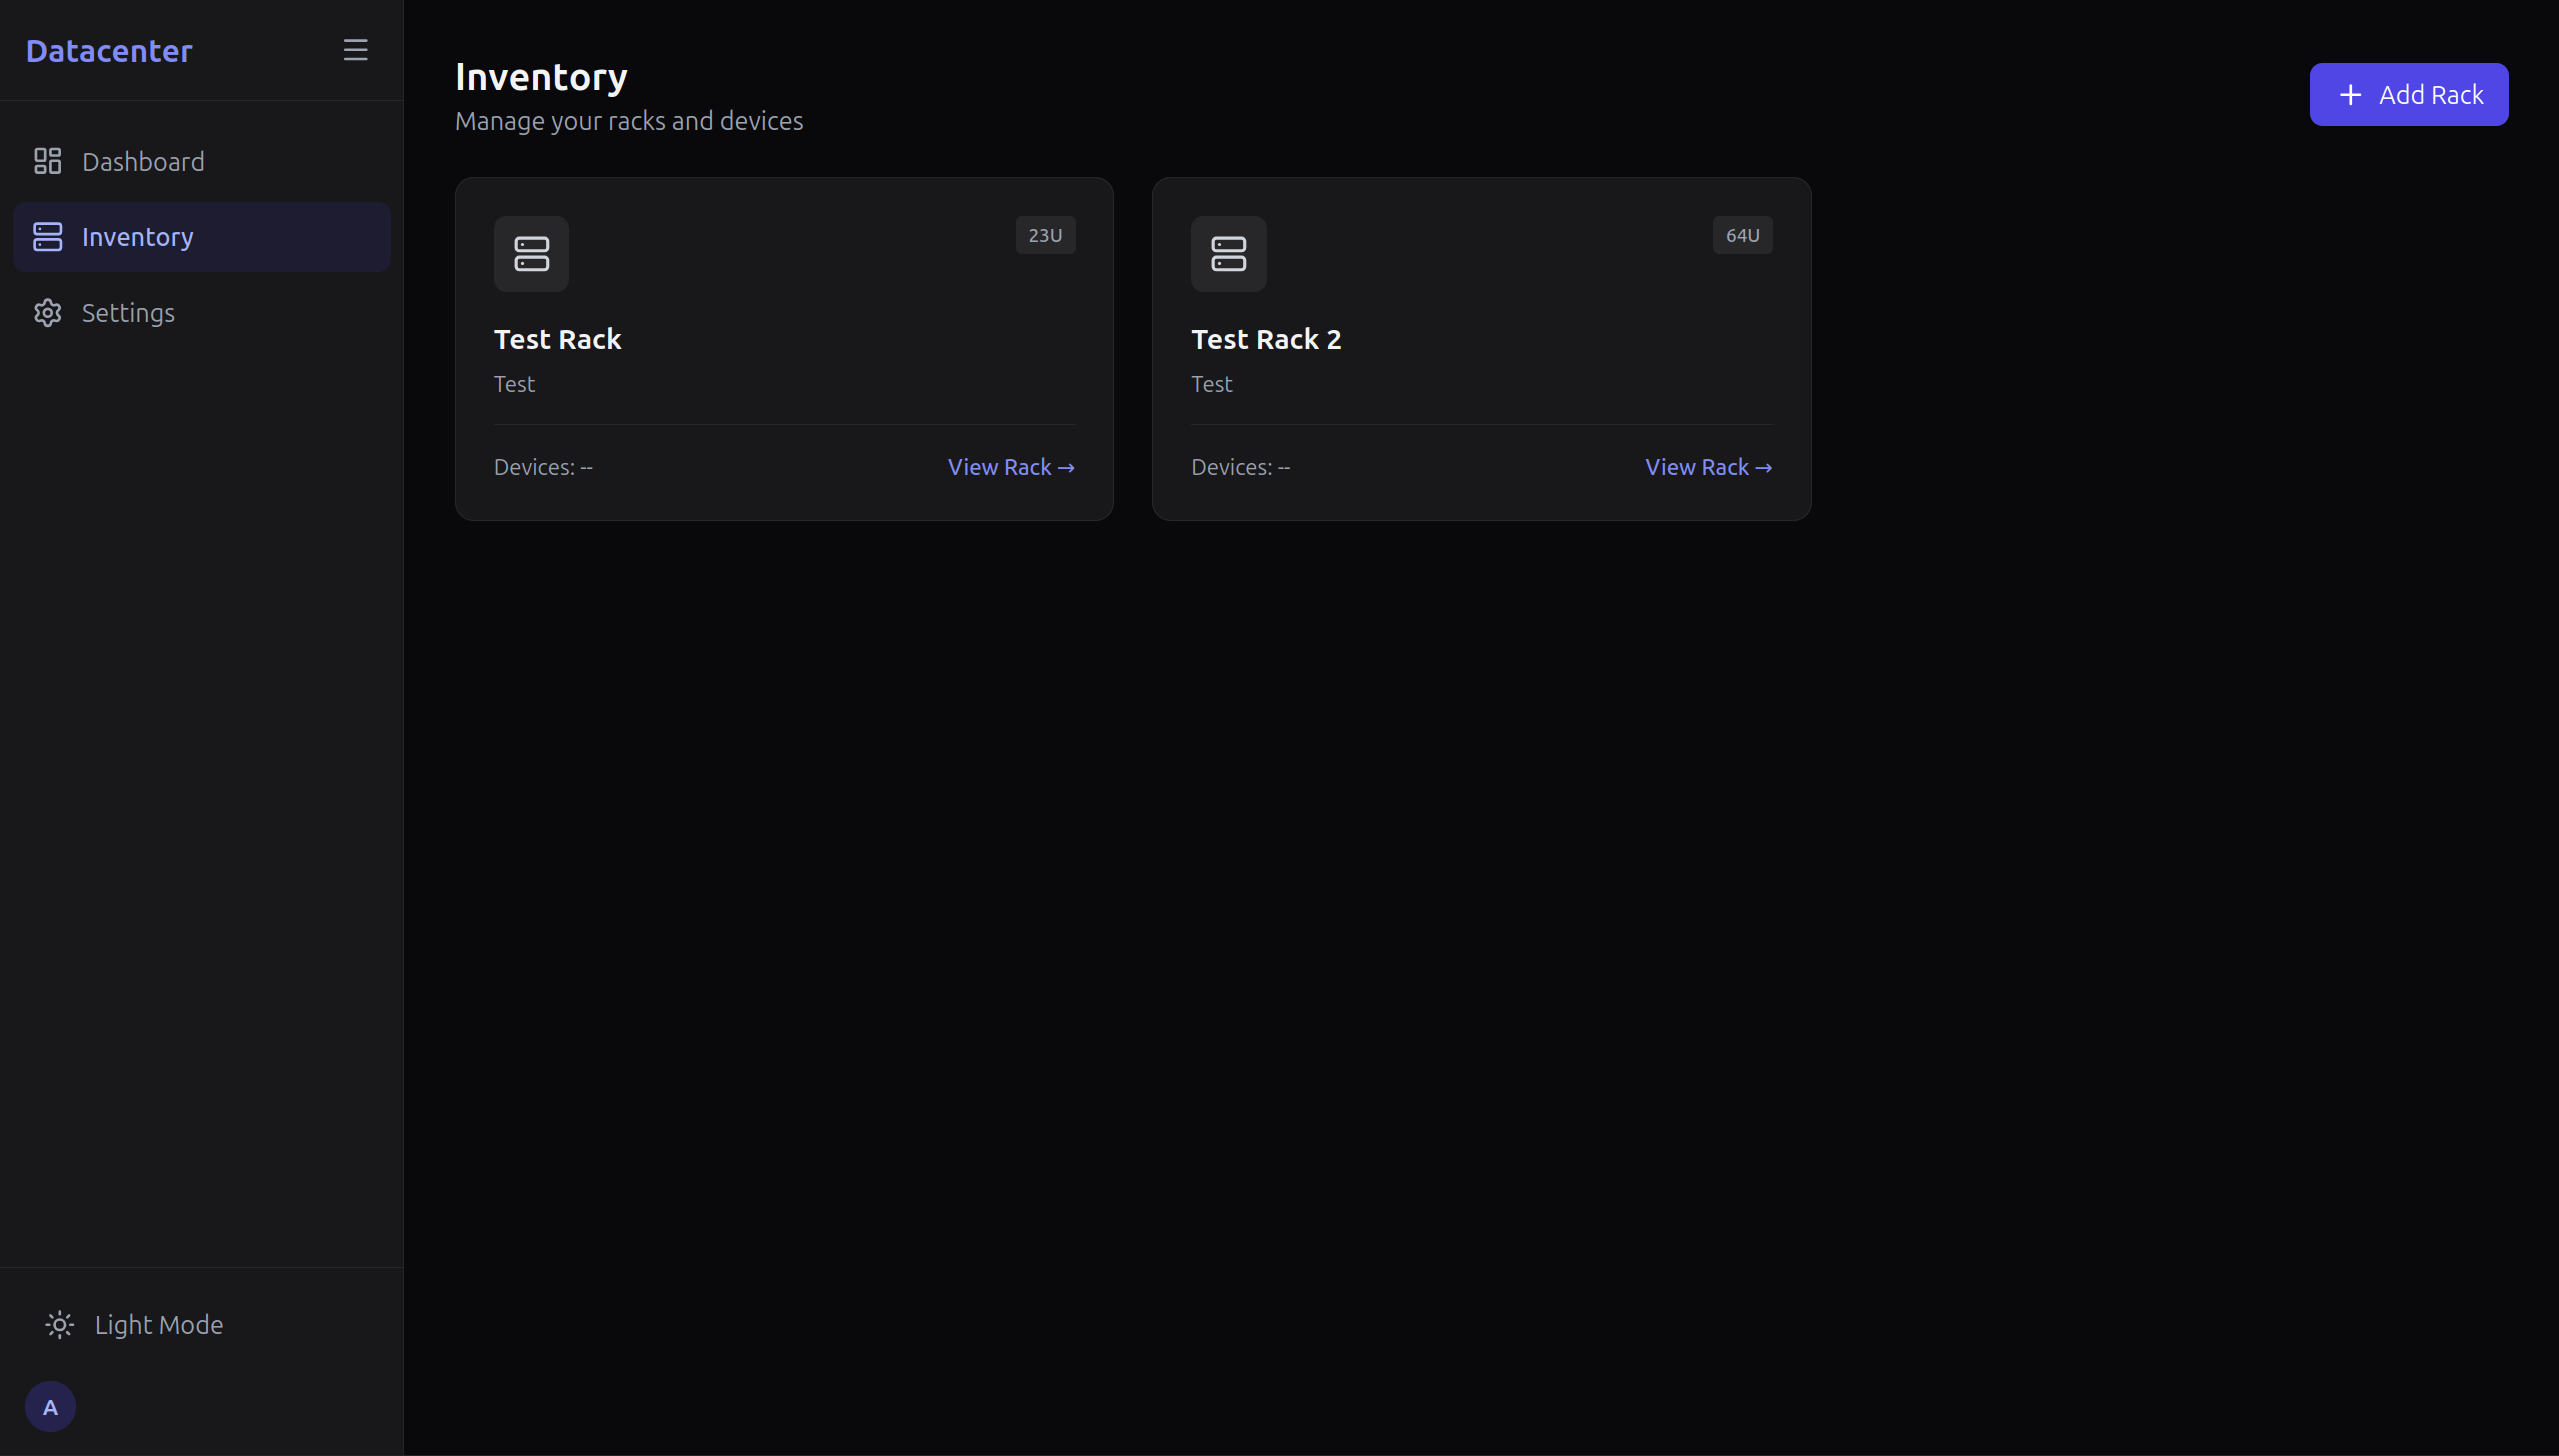
\includegraphics[width=0.95\textwidth]{images/inventory_dash.png}
        \caption{Panoul principal de vizualizare a inventarului (Dashboard)}
        \label{fig:inventory_dash}
    \end{figure}
    
    După cum se observă în Figura~\ref{fig:inventory_dash}, interfața listează rack-urile disponibile sub forma unor "carduri" sintetice, afișând numele rack-ului, locația acestuia și o vizualizare minimizată a gradului de ocupare. Această abordare permite identificarea rapidă a resurselor disponibile fără a fi necesară deschiderea fiecărui rack în parte.
\end{minipage}

\subsubsection{Vizualizarea Detaliată a Rack-ului}
\begin{minipage}{\textwidth}
    Accesând un rack specific, utilizatorul este direcționat către vizualizarea detaliată. Componenta \texttt{RackVisualization} randează o reprezentare fidelă a dulapului metalic, mapând fiecare unitate (U) la starea sa curentă din baza de date.
    
    \begin{figure}[H]
        \centering
        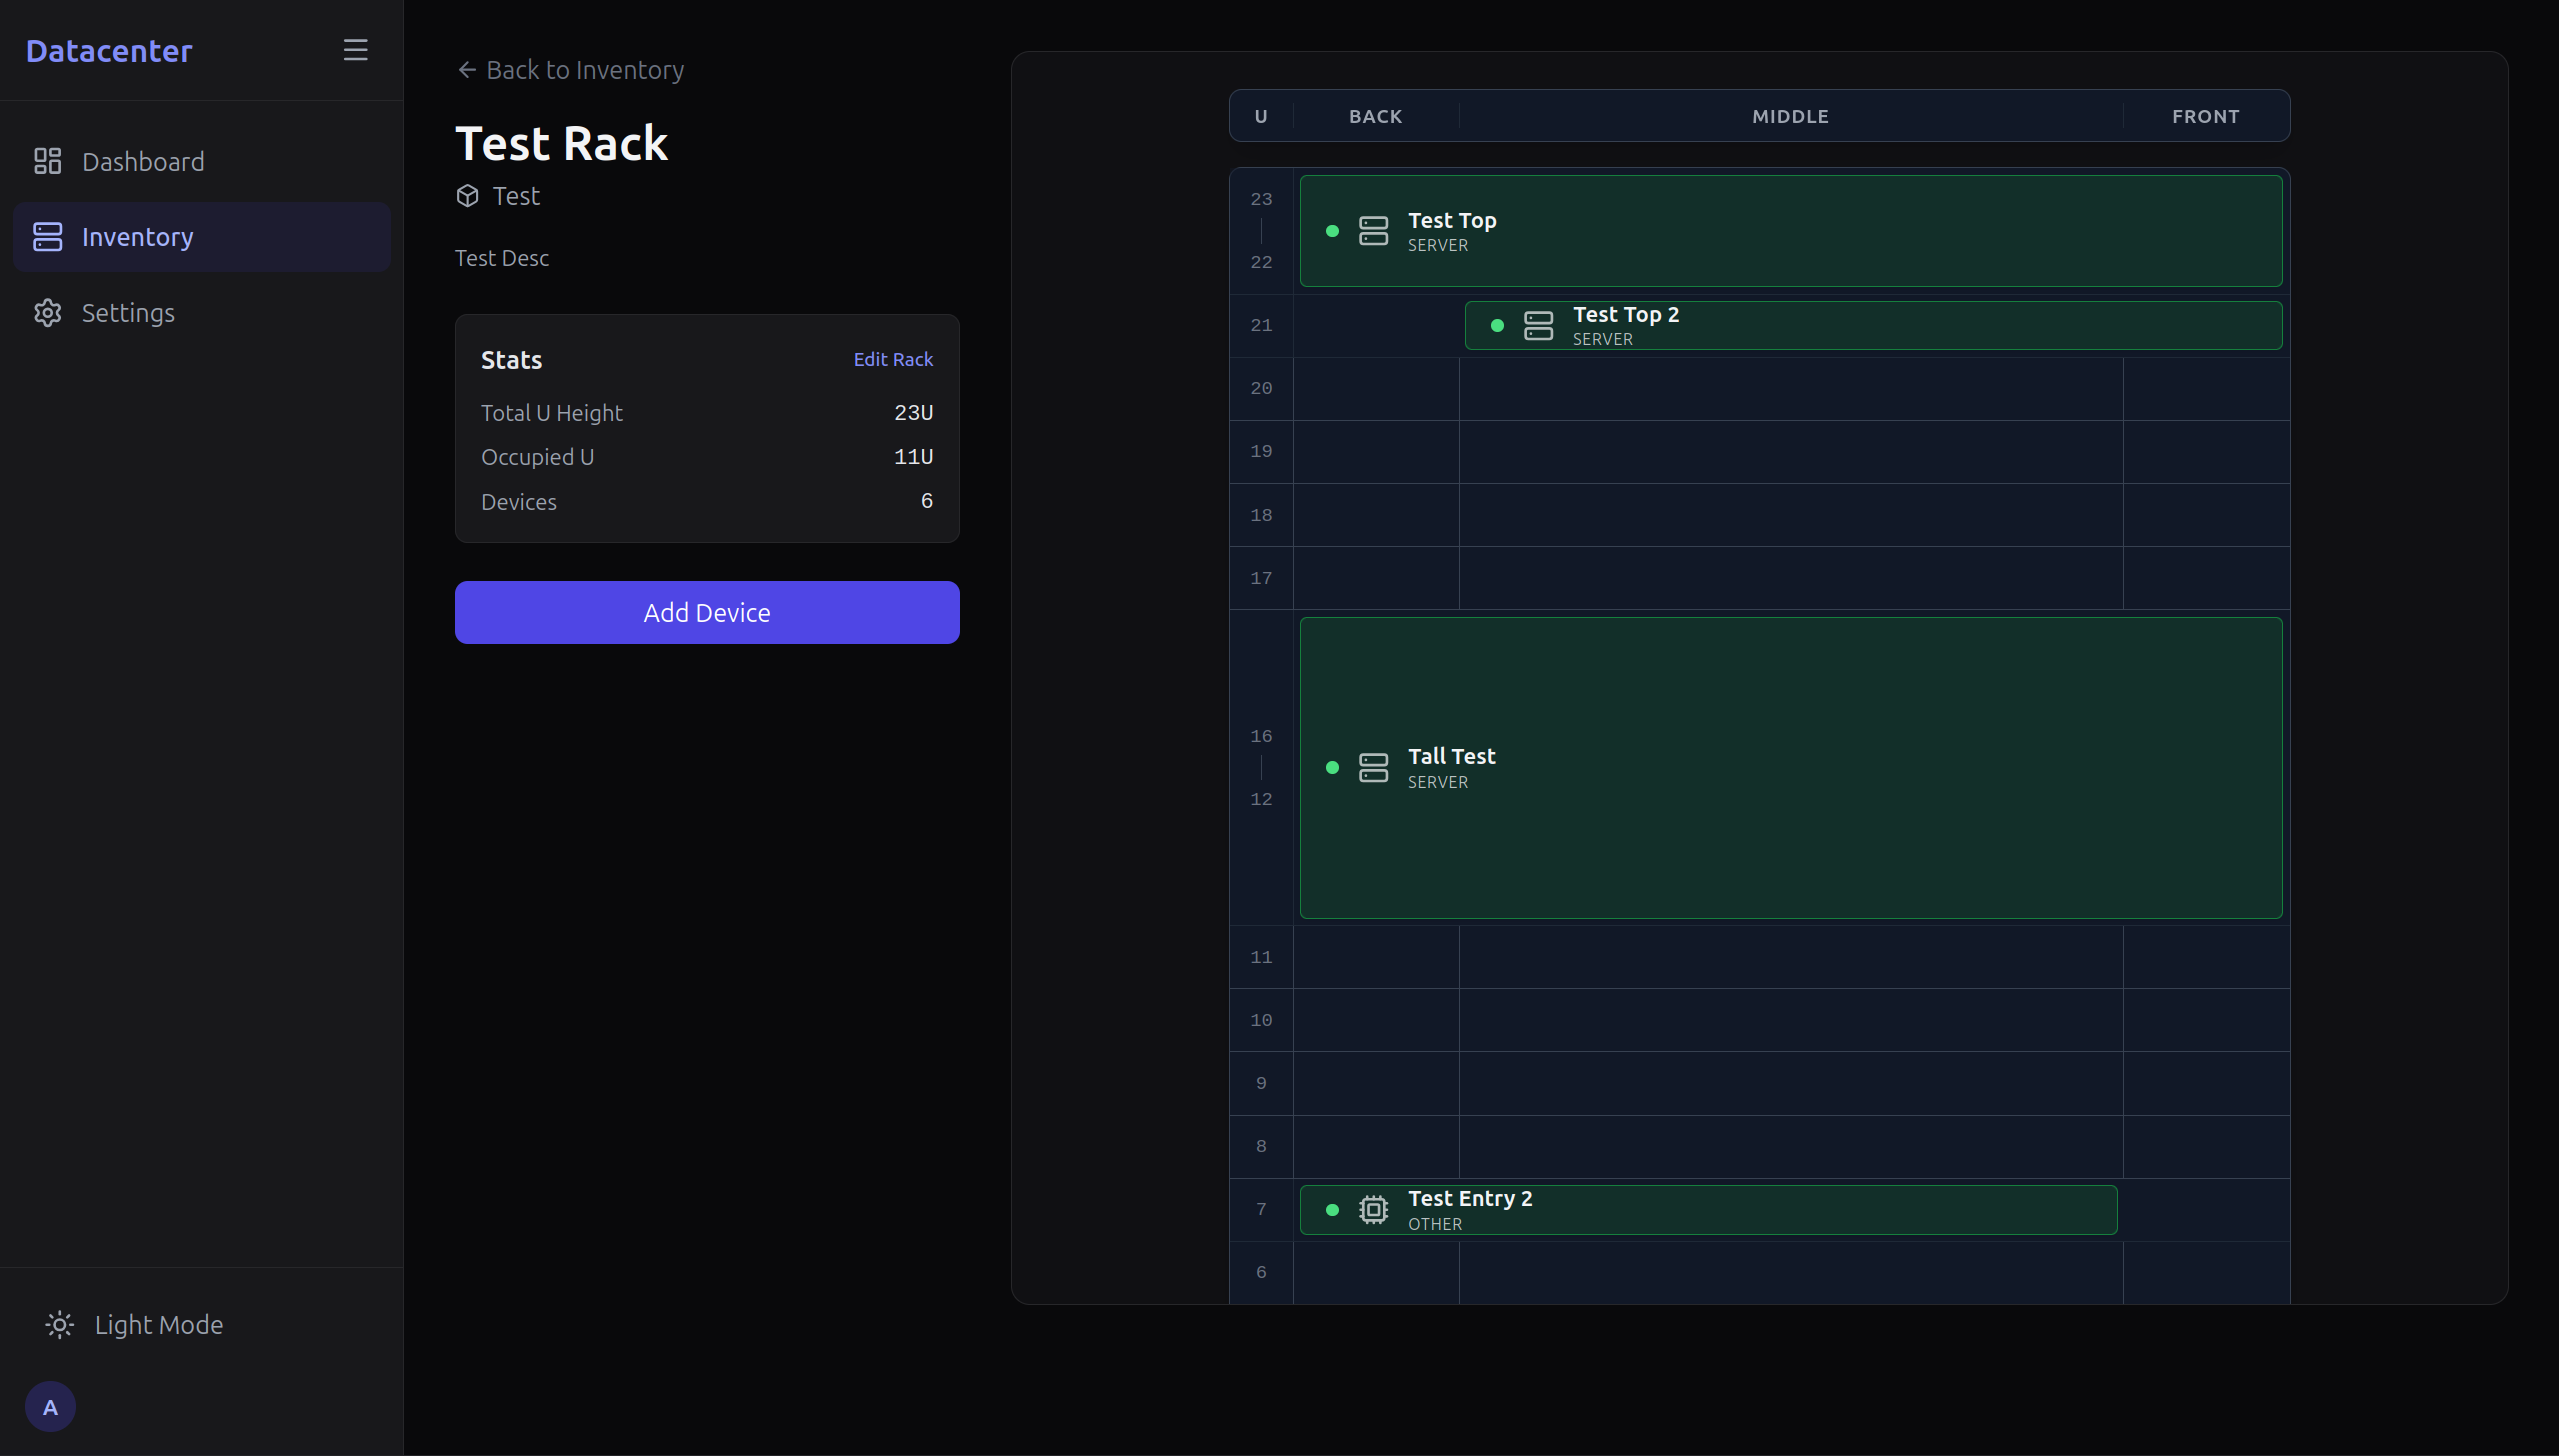
\includegraphics[width=0.95\textwidth]{images/rack_view.png}
        \caption{Vizualizarea grafică detaliată a unui Rack și a echipamentelor instalate}
        \label{fig:rack_view}
    \end{figure}
    
    Figura~\ref{fig:rack_view} ilustrează modul în care echipamentele sunt reprezentate vizual. Dispozitivele care ocupă mai mulți unități (ex: servere 2U sau 4U) sunt randate ca blocuri continue. Codurile de culoare (verde pentru activ, gri pentru inactiv/stocat) și iconițele specifice ajută la distingerea rapidă între diferitele tipuri de echipamente (Switch-uri, Routere, Servere).
    
    Funcționalitatea \textbf{Drag-and-Drop} este activă în această vizualizare: utilizatorul poate selecta un echipament și îl poate muta pe o altă poziție liberă. Sistemul calculează în timp real coliziunile și validează noua poziție, prevenind suprapunerea accidentală a echipamentelor.    
\end{minipage}

\subsubsection{Gestiunea Echipamentelor și a Rack-urilor}

Pentru a adăuga sau modifica resurse, aplicația utilizează ferestre modale (pop-up-uri) care mențin contextul vizual al utilizatorului.

\begin{figure}[H]
    \centering
    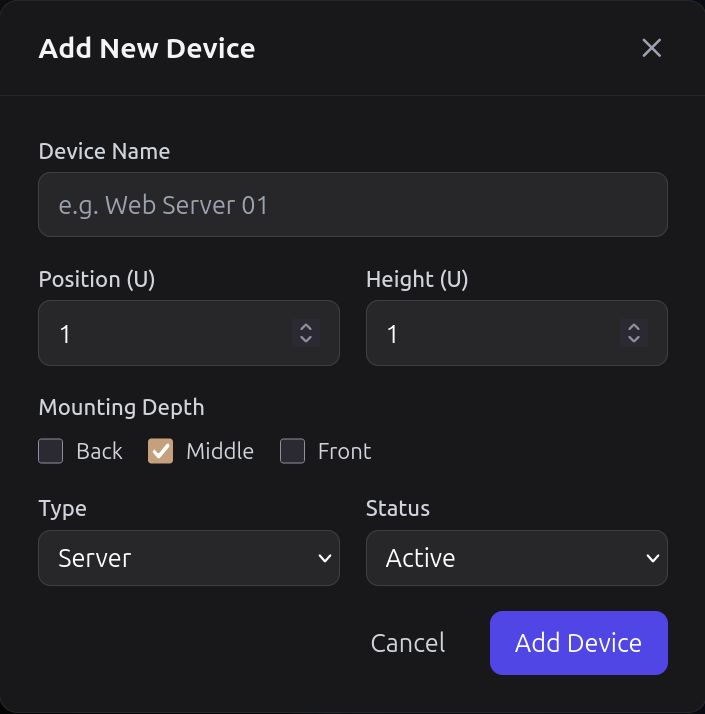
\includegraphics[width=0.7\textwidth]{images/device_add.png}
    \caption{Formularul modal pentru adăugarea unui nou dispozitiv}
    \label{fig:device_add}
\end{figure}

Formularul de adăugare dispozitiv (Figura~\ref{fig:device_add}) permite specificarea detaliilor tehnice esențiale:
\begin{itemize}
    \item \textbf{Nume și Tip:} Identificarea echipamentului.
    \item \textbf{Poziționare:} Înălțimea în U și poziția de start.
    \item \textbf{Configurație Montare:} Specificarea dacă echipamentul este montat în fața sau în spatele rack-ului, un detaliu critic pentru managementul termic și al cablării.
\end{itemize}

Similar, editarea proprietăților unui Rack se realizează printr-o interfață dedicată (Figura~\ref{fig:rack_edit}), permițând redenumirea sau schimbarea dimensiunilor acestuia.

\begin{figure}[H]
    \centering
    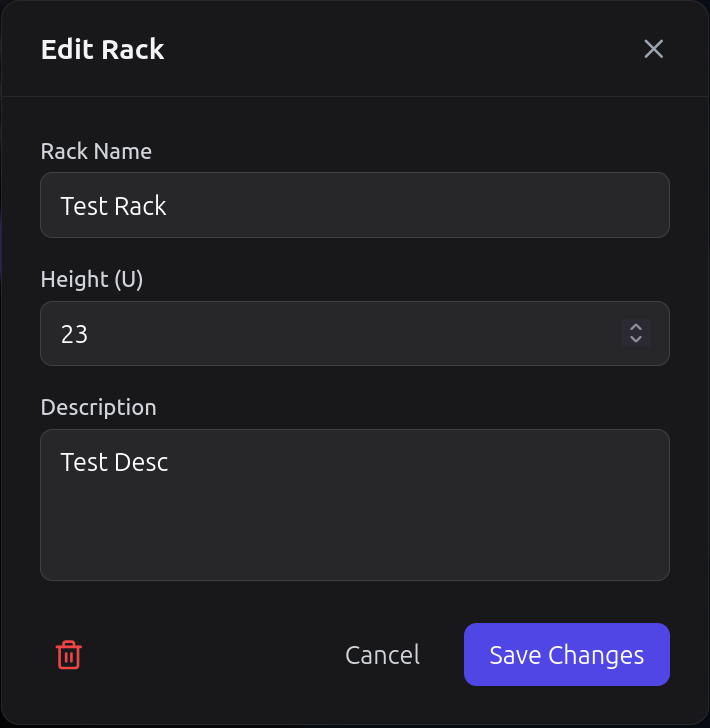
\includegraphics[width=0.7\textwidth]{images/rack_edit.png}
    \caption{Interfața de editare a proprietăților unui Rack}
    \label{fig:rack_edit}
\end{figure}

\subsection{Structura Backend-ului (Django)}

Backend-ul aplicației asigură integritatea datelor și expune API-ul necesar frontend-ului. Structura proiectului Django este organizată modular, aplicația \texttt{inventory} fiind responsabilă de logica de business.

\subsubsection{Modelele de Date}

Transpunerea conceptelor fizice în structuri de date s-a realizat prin utilizarea modelor Django. 

\begin{lstlisting}[language=Python, caption={Definirea modelului Device în Django}, label={lst:device_model}]
class Device(models.Model):
    DEVICE_TYPES = [
        ('server', 'Server'),
        ('switch', 'Switch'),
        ('router', 'Router'),
        ('pdu', 'PDU'),
        ('other', 'Other'),
    ]

    name = models.CharField(max_length=100)
    rack = models.ForeignKey(Rack, on_delete=models.CASCADE, related_name='devices')
    position_u = models.PositiveIntegerField(help_text="Bottom-most U position")
    height_u = models.PositiveIntegerField(default=1)
    
    # Configurare flexibilă pentru montare (JSON)
    mounting_configuration = models.JSONField(default=list)
    
    status = models.CharField(max_length=50, choices=STATUS_CHOICES, default='active')
    specs = models.JSONField(default=dict, blank=True)
\end{lstlisting}

Utilizarea câmpurilor \texttt{JSONField} pentru specificații și configurarea montării oferă flexibilitatea necesară pentru a acomoda diverse tipuri de echipamente fără a modifica schema bazei de date pentru fiecare nou atribut.

\subsection{Validarea Regimului de Poziționare}

O componentă critică a implementării este logica de validare a poziționării. Spre deosebire de un simplu tabel, un rack fizic are constrângeri spațiale stricte. Backend-ul implementează verificări riguroase înainte de a salva orice modificare:

\begin{enumerate}
    \item \textbf{Validarea Limitelor:} Se verifică dacă echipamentul "încape" fizic în rack (ex: un server de 4U nu poate fi montat la poziția 40 într-un rack de 42U).
    \item \textbf{Detectarea Coliziunilor:} Se interoghează baza de date pentru a găsi orice alt echipament care ocupă intervalul $[pozitie\_start, pozitie\_start + inaltime]$. Dacă intersecția este nevidă, operațiunea este respinsă.
\end{enumerate}

Această dublă validare (în Frontend pentru UX și în Backend pentru consistență) asigură robustețea sistemului și previne coruperea datelor de inventar.

\newpage
\section{Concluzii și Direcții Viitoare}
\label{sec:concluzii}

Sistemul dezvoltat reprezintă o soluție modernă și eficientă pentru digitalizarea inventarului în centrele de date. Prin combinarea unei interfețe vizuale interactive cu un backend solid, aplicația rezolvă problemele de acuratețe și vizibilitate întâlnite în metodele tradiționale de gestiune.

Arhitectura modulară bazată pe Microservicii (containere Docker) asigură ușurința în instalare cât și scalabilitatea necesară pentru extinderi viitoare.

Direcțiile viitoare de cercetare și dezvoltare includ:
\begin{itemize}
    \item \textbf{Monitorizare Activă:} Integrarea cu protocoale SNMP pentru a prelua date în timp real (temperatură, consum) direct de la echipamente.
    \item \textbf{Planificare Capacitate:} Implementarea unor algoritmi care să sugereze automat locația optimă pentru instalarea noilor echipamente, bazat pe spațiul și puterea disponibilă.
    \item \textbf{Versiunea Mobilă:} Adaptarea interfeței pentru tablete, permițând tehnicienilor să actualizeze inventarul direct din fața rack-ului.
\end{itemize}

% ============================================================================
% BIBLIOGRAPHY
% ============================================================================

\newpage
\phantomsection
\addcontentsline{toc}{section}{Bibliografie}
\begin{thebibliography}{9}

\bibitem{ralph}
Allegro,
\newblock \emph{Ralph: ``a simple yet powerful Asset Management, DCIM and CMDB system for data center and back office.''},
\newblock Open-source software, \url{https://github.com/allegro/ralph/}

\bibitem{racktables}
RackTables Developers, 
\newblock \emph{RackTables: ``a nifty and robust solution for datacenter and server room asset management.''},
\newblock Open-source software, \url{https://www.racktables.org/}

\bibitem{netbox}
NetBox Labs,
\newblock \emph{NetBox: The premier source of truth powering network automation},
\newblock Open-source software, \url{https://netboxlabs.com/products/netbox/}

\bibitem{opendcim}
openDCIM Foundation,
\newblock \emph{openDCIM: An open source (GPL v3) Data Center Inventory Management (DCIM) application}
\newblock Open-source software, \url{https://opendcim.org/}

\end{thebibliography}

% ============================================================================
% APPENDICES (optional)
% ============================================================================

% \appendix
% \section{Anexe}
% \label{sec:anexe}

% Conținut anexe aici...

\end{document}